% AAAI-format paper (js3cnet) - decompiled from PDF
% Use article + twocolumn when aaai.sty is not available
\documentclass[11pt,twocolumn]{article}
\usepackage[utf8]{inputenc}
\usepackage[T1]{fontenc}
\usepackage[margin=1in]{geometry}
\usepackage{amsmath,amssymb,amsfonts}
\usepackage{graphicx}
\usepackage{booktabs}
\usepackage{subcaption}
\usepackage{cite}
\usepackage{hyperref}
\usepackage{url}

\DeclareMathOperator*{\argmax}{arg\,max}
\DeclareMathOperator*{\argmin}{arg\,min}

\title{Sparse Single Sweep LiDAR Point Cloud Segmentation via Learning Contextual Shape Priors from Scene Completion}
\author{
  Xu Yan$^{1,2}$\textsuperscript{\dagger}, Jiantao Gao$^{2,4}$\textsuperscript{\dagger}, Jie Li$^{1,3}$, Ruimao Zhang$^{1,2}$, Zhen Li$^{1,2}$*,\\
  Rui Huang$^{1,3}$, Shuguang Cui$^{1,2}$\\
  \small $^1$The Chinese University of Hong Kong (Shenzhen), $^2$Shenzhen Research Institute of Big Data,\\
  \small $^3$Shenzhen Institute of Artificial Intelligence and Robotics for Society, $^4$Shanghai University\\
  \small \{xuyan1@link., lizhen@\}cuhk.edu.cn\\
  \small *Corresponding author. \textsuperscript{\dagger}Equal first authorship.
}
\date{}

\begin{document}
\maketitle

\begin{abstract}
LiDAR point cloud analysis is a core task for 3D computer vision, especially for autonomous driving. However, due to the severe sparsity and noise interference in the single sweep LiDAR point cloud, the accurate semantic segmentation is non-trivial to achieve. In this paper, we propose a novel sparse LiDAR point cloud semantic segmentation framework assisted by learned contextual shape priors. In practice, an initial semantic segmentation (SS) of a single sweep point cloud can be achieved by any appealing network and then flows into the semantic scene completion (SSC) module as the input. By merging multiple frames in the LiDAR sequence as supervision, the optimized SSC module has learned the contextual shape priors from sequential LiDAR data, completing the sparse single sweep point cloud to the dense one. Thus, it inherently improves SS optimization through fully end-to-end training. Besides, a Point-Voxel Interaction (PVI) module is proposed to further enhance the knowledge fusion between SS and SSC tasks. Furthermore, the auxiliary SSC and PVI modules can be discarded during inference without extra burden for SS. Extensive experiments confirm that our JS3C-Net achieves superior performance on both SemanticKITTI and SemanticPOSS benchmarks, i.e., 4\% and 3\% improvement correspondingly.
\end{abstract}

\section{Introduction}
\label{sec:intro}

LiDAR point clouds, compared with data from other sensors such as cameras and radars in autonomous driving perception, have advantages of both accurate distance measurements and fine semantic descriptions. Semantic segmentation of LiDAR point clouds is usually conducted by assigning a semantic class label to each point. It is traditionally viewed as a typical task in the computer vision community. In autonomous driving, accurate and effective point cloud semantic segmentation undoubtedly plays a critical role.

Previous studies \cite{thomas2019,wu2019} about point cloud semantic segmentation mainly focused on the complete or dense point cloud scenarios, which are post-processed by merging multiple collected LiDAR or RGB-D sequences (e.g., ScanNet \cite{dai2017}, S3DIS \cite{armeni2017} and Semantic3D \cite{riegler2017}). However, raw per-sweep LiDAR point clouds, as the original input of autonomous driving, are much sparser. Their sparsity usually increases with the reflection distance, which often leads to extremely shapes missing and uneven point sampling for various categories. Therefore, despite the promising performance on complete data (e.g., 80\% mIOU on Semantic3D), the semantic segmentation of sparse single sweep LiDAR point cloud still remains a big challenge, which extremely limits its accuracy in real applications.

In this paper, we try to break through the barrier of semantic segmentation on sparse single sweep LiDAR point clouds. One plausible way is to fully utilize the sequential nature of LiDAR data. Taking the scenario shown in Fig.~\ref{fig:1} as an example, for a per-sweep point cloud with extremely sparse points of the truck, it seems impossible for previous methods to conduct accurate segmentation. Nevertheless, such segmentation would be possible if we introduce the richer shape information from the other two frames (Fig.~\ref{fig:1}(b) and (c)) to reconstruct a shape-complete truck as shown in Fig.~\ref{fig:1}(d). For this purpose, some previous works utilized historical adjacent frames to supplement the local details missing from the point clouds. For instance, SpSequenceNet \cite{shi2020} and MeteorNet \cite{liu2019} use the point cloud of the current frame to query the nearest neighbors from the previous frames, following which a feature aggregation is conducted to fuse the adjacent-frame information. PointRNN \cite{fan2019} applies Recurrent Neural Networks (RNNs) to select available features from previous scenes. However, all of the above methods become unavailable in most real scenarios since: (1) These methods exclusively use historical frames of the current scene in LiDAR sequence; (2) Their proposed feature aggregation methods inevitably increase the computational burden.

To solve the above issues, we propose an enhanced Joint single sweep LiDAR point cloud Semantic Segmentation by exploiting learned shape prior from Scene Completion network, i.e., JS3C-Net. Specifically, by merging dozens of consecutive frames in a LiDAR sequence, a large complete point cloud is achieved as ground truth for the Semantic Scene Completion (SSC) task without extra annotation. The optimized SSC by using these annotations could capture the compelling shape priors. Furthermore, a well-designed Point-Voxel Interaction (PVI) module is proposed for implicit mutual knowledge fusion between the SS and SSC tasks. More importantly, we design our SSC and PVI modules to be disposable. Our main contributions are: (1) JS3C-Net is the first to achieve the enhanced sparse single sweep LiDAR semantic segmentation via auxiliary scene completion; (2) For better trade-off, our auxiliary components are designed in cascaded and disposable manners, and a novel PVI module is proposed; (3) Our method shows superior results on both SS and SSC on SemanticKITTI \cite{kendall2018} and SemanticPOSS \cite{pan2020}.

\begin{figure}[t]
\centering

\includegraphics[width=0.24\textwidth]{figures/fig_1_1}\quad

\includegraphics[width=0.24\textwidth]{figures/fig_1_2}\quad
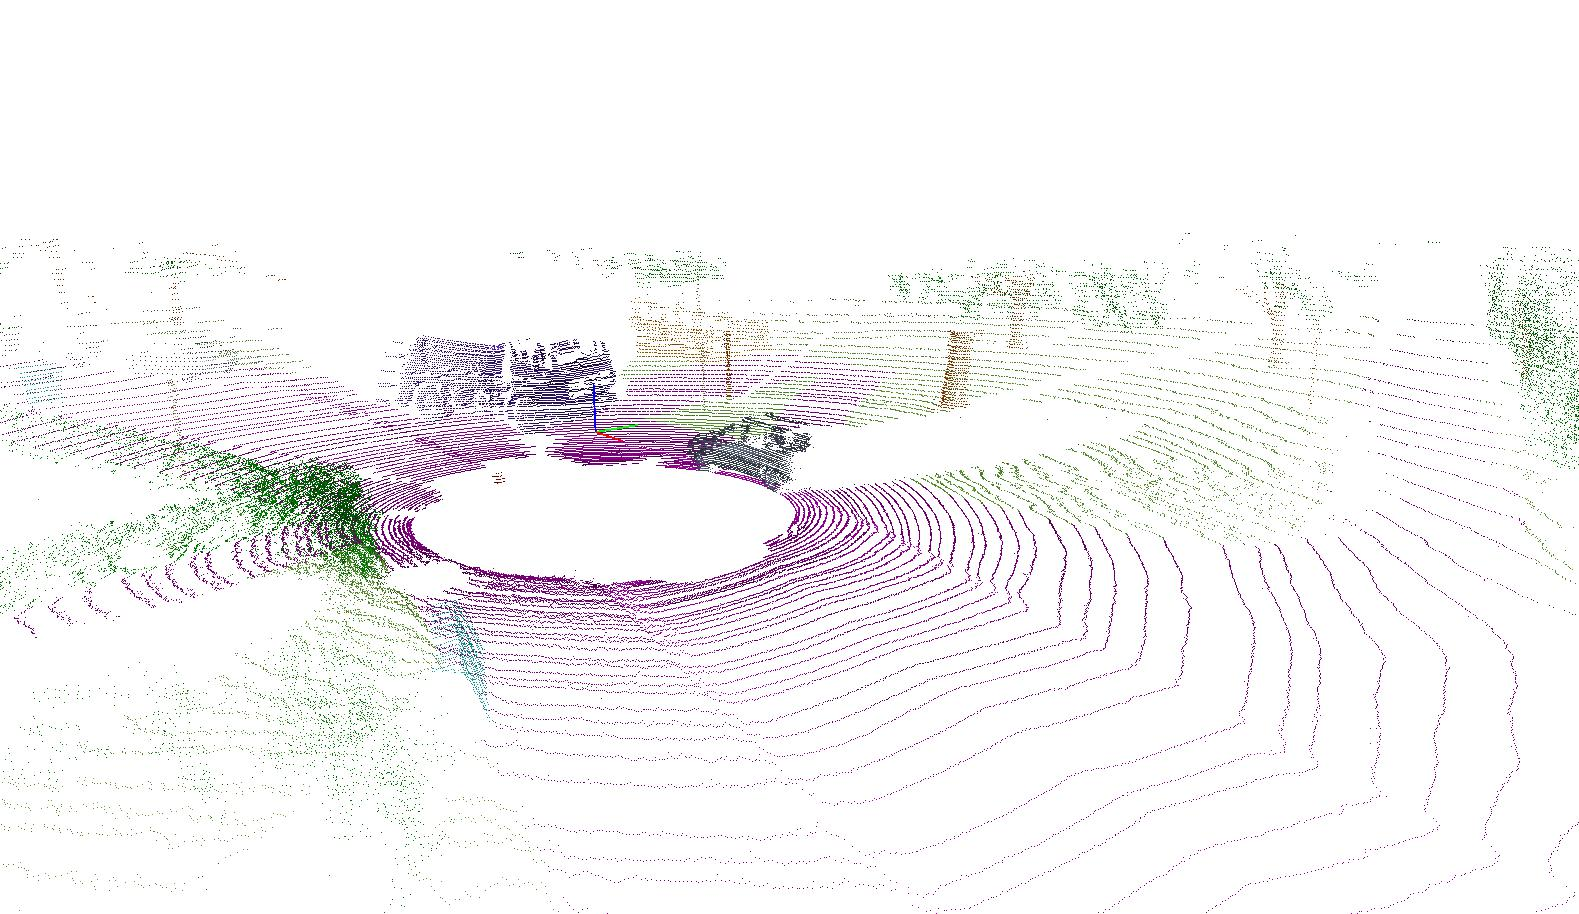
\includegraphics[width=0.24\textwidth]{figures/fig_1_3}\quad
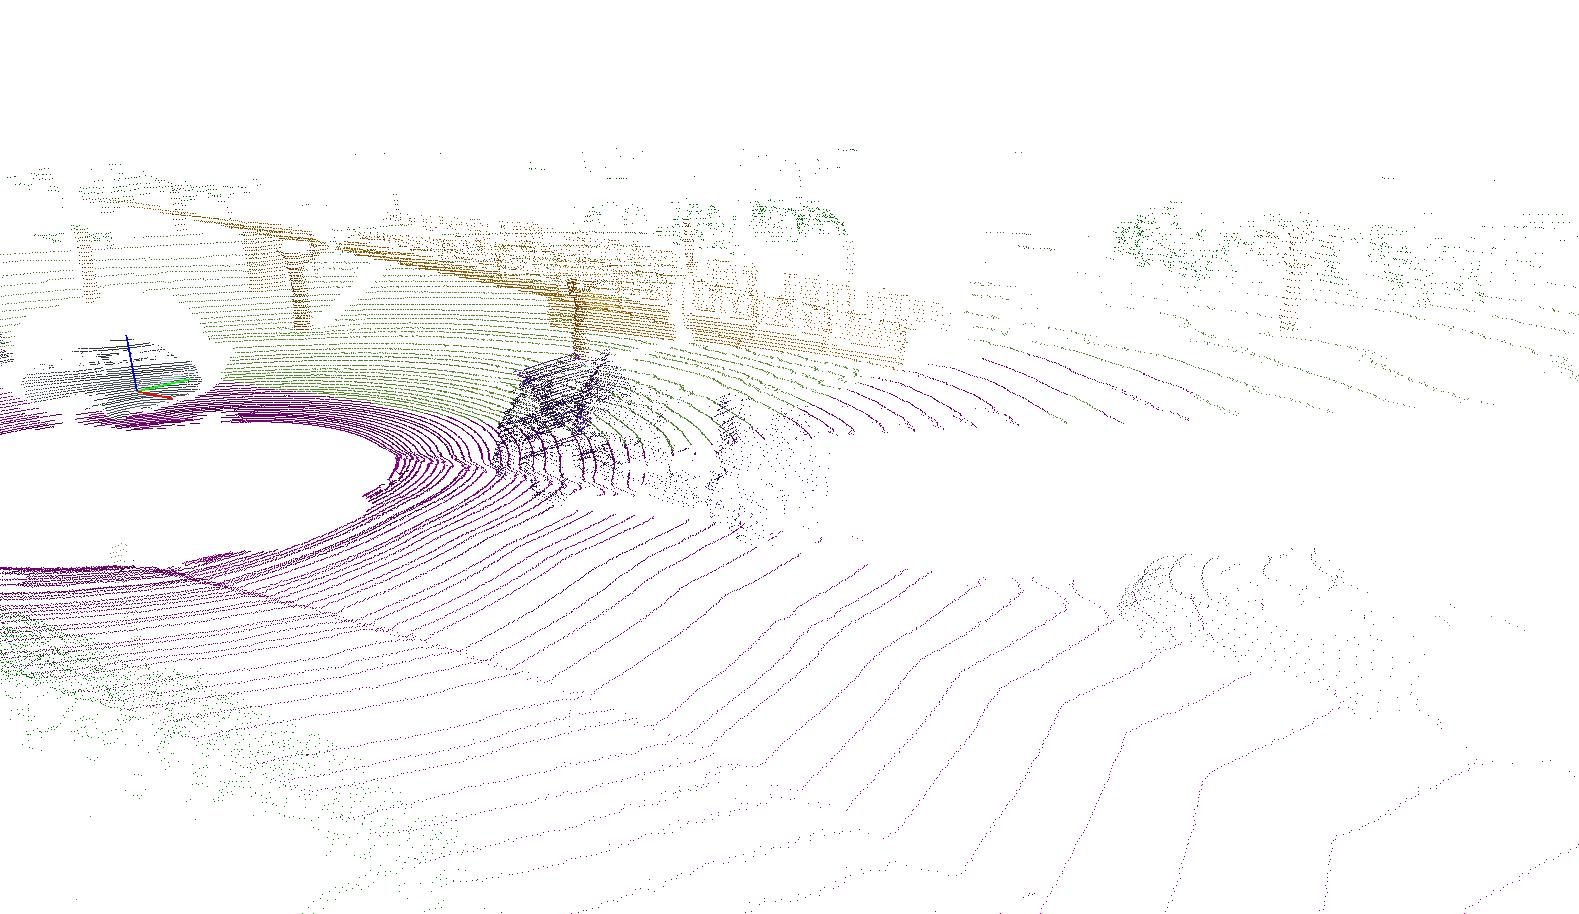
\includegraphics[width=0.24\textwidth]{figures/fig_1_4}
\caption{Learning shape priors from multiple frames. For the sparse per-sweep point cloud shown in (a), it is non-trivial for current methods to recognize the truck from partial components. However, if we introduce the auxiliary information from adjacent frames (b) and (c), it is much easier to segment the complete truck in (d).}
\label{fig:1}
\end{figure}

\section{Related Work}
\label{sec:related}

\textbf{Point Cloud Semantic Segmentation.} Unlike 2D images with regular grids, point clouds are often sparse and disordered. There are three main strategies: (1) Projection-based methods map point clouds onto 2D pixels so that traditional CNN can play a normal role \cite{landrieu2019}; (2) Voxel-based methods use efficient spatial sparse convolution \cite{liu2018} and octree based networks \cite{ronneberger2015}; (3) Point-based methods directly process raw point clouds \cite{xu2020,yan2020}. However, previous methods often suffer from local information missing in LiDAR scenes due to insufficient priors and bias in data collection.

\textbf{Semantic Scene Completion.} SSC aims to produce a complete 3D voxel representation from an incomplete input. Song et al. \cite{song2017} firstly use single-view depth as input to construct SSCNet. Spatially sparse group convolution is used in \cite{zhang2018} for fast 3D dense prediction.

\textbf{Multi-task Learning.} Multi-task learning aims to improve the learning efficiency and prediction accuracy through knowledge transfer. OccuSeg \cite{han2020} proposes a 3D voxel projection-based segmentation network. However, the shape priors brought by completion tasks are often neglected in previous works.

\section{Method}
\label{sec:method}

The pipeline of JS3C-Net is illustrated in Fig.~\ref{fig:2}. We first use a general point cloud segmentation network to obtain initial point semantic segmentation and a shape embedding (SE) for each incomplete single-frame point cloud. Then the SSC module takes results of the segmentation network as input and generates the completed voxel of the whole scene with dense convolution neural network. Meanwhile, a Point-Voxel Interaction (PVI) module is proposed to conduct shape-aware knowledge transfer.

\subsection{Semantic Segmentation}
In general, a point cloud has two components: the points $\mathbf{P} \in \mathbb{R}^{N \times 3}$ and their features $\mathbf{F} \in \mathbb{R}^{N \times D}$. We simply choose Submanifold SparseConv as our backbone. The voxel-based output from sparse convolution U-Net is transformed back to point-wise features $F_{\mathrm{enc}} \in \mathbb{R}^{N \times F}$ by nearest-neighbor interpolation. We use multi-layer perceptions (MLP$_1$) to transfer their features to shape embedding $F_{\mathrm{SE}} \in \mathbb{R}^{N \times D_e}$, which works as the input of the subsequent point-voxel interaction module. Finally, $F_{\mathrm{out}} \in \mathbb{R}^{N \times C}$ are the outputs for point cloud semantic segmentation.

\subsection{Cascaded Semantic Scene Completion}
The SSC module aims to introduce contextual shape priors from the entire LiDAR sequence. It takes the semantic probability $F_{\mathrm{out}}$ from the SparseConv as input, and then predicts the completion results. The architecture uses voxelization, convolution layers, basic blocks with skip-connection, and dense upsampling to obtain a voxel output with $C+1$ channels.

\subsection{Shape-aware Point-Voxel Interaction}
To fully utilize implicit knowledge transfer for mutual improvements of two tasks, we propose a shape-aware PVI module. Per point shape embedding $F_{\mathrm{SE}}$ and coarse completion from the SSC module flow into PVI as input. PVI firstly selects geometric centers of all non-empty voxels, then uses $k$-nearest neighbor by Euclidean distance to query the closest points from the original point cloud $\mathbf{P}$. A graph convolutional network is employed to enhance the relation learning. We adopt the convolutional operator from DGCNN to define edge-features $e_{ij}$ between two points as
\begin{equation}
e_{ij} = \phi([p^v_i, f^v_i], [p^v_i, f^v_i] - [p_j, f_j]),
\end{equation}
where $f^v$ and $f$ are features of point $p^v$ and $p$ respectively, and $[\cdot,\cdot]$ means concatenation. Finally, this enhanced feature is added to the original coarse completion output through a residual connection.

\subsection{Uncertainty-weighted Multi-task Loss}
We use the uncertainty weighting method proposed in \cite{kendall2018}. The joint loss can be written as
\begin{equation}
\mathcal{L}(W, \sigma_1, \sigma_2) = \frac{1}{2\sigma_1^2} \mathcal{L}_{\mathrm{seg}}(W_{\mathrm{seg}}) + \frac{1}{2\sigma_2^2} \mathcal{L}_{\mathrm{complet}}(W) + \log \sigma_1 + \log \sigma_2,
\end{equation}
where $\mathcal{L}_{\mathrm{seg}}$ and $\mathcal{L}_{\mathrm{complet}}$ are weighted cross-entropy losses.

\begin{figure}[t]
\centering

\includegraphics[width=\textwidth]{figures/fig_4_35}
\caption{Overall pipeline of JS3C-Net. The SSC and PVI modules can be discarded during inference.}
\label{fig:2}
\end{figure}

\section{Experiments}
\label{sec:exp}

We evaluate JS3C-Net on SemanticKITTI \cite{kendall2018} and SemanticPOSS \cite{pan2020}. We merge consecutive 70 frames for every single frame to generate the complete volume. We select a volume of 51.2m in front of the LiDAR, 25.6m to each side, and 6.4m in height with resolution 0.2m, resulting in $256 \times 256 \times 32$ voxels. We use the Adam optimizer, batch size 6, 50 epochs, initial learning rate 0.001 (decreased by 30\% every 5 epochs).

\subsection{Semantic Segmentation}
As shown in the results, our JS3C-Net surpasses all existing methods by a large margin. JS3C-Net achieves significant improvements on small objects (e.g., motorcycle, bicycle). Thanks to the contextual shape priors from SSC, our JS3C-Net can segment them well.

\begin{figure}[t]
\centering
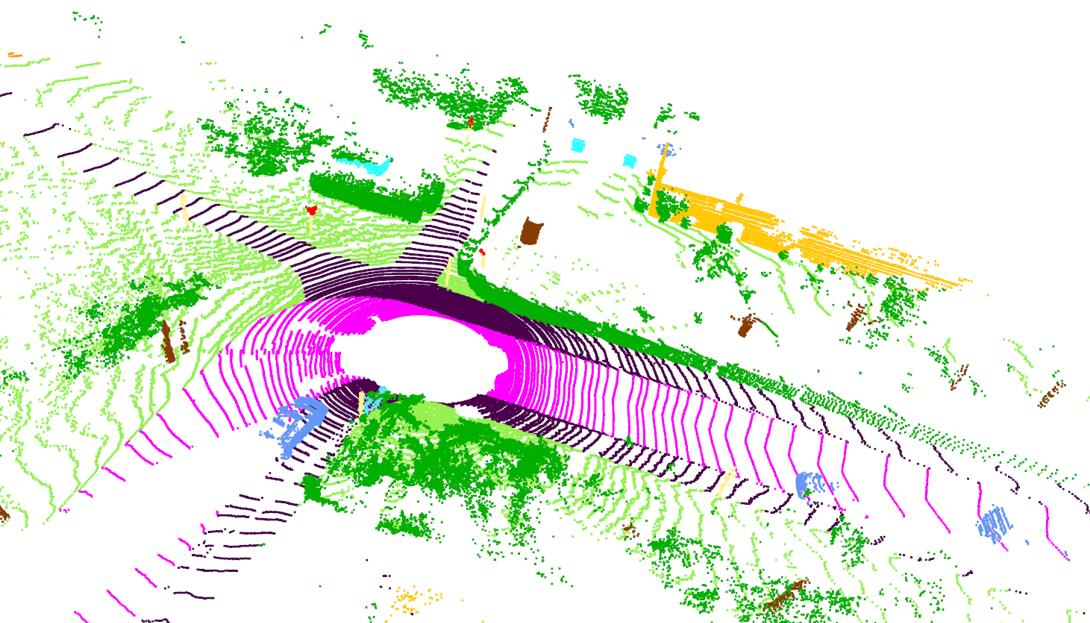
\includegraphics[width=\textwidth]{figures/fig_6_1}
\caption{Qualitative results of JS3C-Net on the validation set of SemanticKITTI.}
\label{fig:4}
\end{figure}

\subsection{Semantic Scene Completion}
With the semantic guidance from the segmentation network, our JS3C-Net can also make significant breakthrough in semantic scene completion. Our results are 6\% higher than previous state-of-the-art TS3D3 for scene completion.

\subsection{Ablation Study}
The baseline (model A) is set to learn without joint learning. The baseline only gets IoU of 63.1\% on SS and 51.1\% on SC. Model B with joint learning improves to 66.1\% for SS and 55.0\% for SC. Model C with uncertainty multi-task loss further improves. With the PVI module, our JS3C-Net achieves the best results on both tasks.

\subsection{Complexity Analysis}
Our JS3C-Net is much more light-weighted and faster than previous point-based methods. Since the disposable properties of our SSC and PVI modules, JS3C-Net has the same speed with the segmentation backbone during inference.

\section{Conclusion}
\label{sec:conclusion}

In this work, we propose a single sweep LiDAR point cloud semantic segmentation framework via contextual shape priors from semantic scene completion network, named JS3C-Net. By exploiting sophisticated pipelines, interactive modules, and reasonable loss function, our JS3C-Net model achieves state-of-the-art results on both semantic segmentation and scene completion tasks, outperforming previous methods by a large margin. We believe that our work can be applied to a wider range of other scenarios in the future. Meanwhile, our method provides an alternative solution to the comprehension of large-scale LiDAR scenes with severe local details missing.

\section*{Acknowledgments}
The work was supported in part by the Key Area R\&D Program of Guangdong Province (No.2018B030338001), the National Key R\&D Program of China (No.2018YFB1800800), NSFC-Youth 61902335, Guangdong Regional Joint Fund-Key Projects 2019B1515120039, Shenzhen Outstanding Talents Training Fund, Shenzhen Institute of Artificial Intelligence and Robotics for Society, Guangdong Research Project No.2017ZT07X152 and CCF-Tencent Open Fund.

\bibliographystyle{plain}
\bibliography{references}

\end{document}
